% !TeX program = xelatex
\documentclass[12pt,a4paper]{exam-zh}

\usepackage{amsmath,array,graphicx,booktabs,multirow}
\usepackage{enumitem}
\usepackage{fancyhdr}
\usepackage{tikz}
\usepackage{tabularx}
\usepackage{setspace}
\setCJKmainfont{Noto Serif CJK SC}
\geometry{margin=2.2cm,top=2.0cm,bottom=2.2cm}
\pagestyle{fancy}
\fancyhf{}
\cfoot{-\thepage{}-}
\renewcommand{\headrulewidth}{0pt}
\renewcommand{\footrulewidth}{0pt}
\setlength{\parindent}{0pt}
\setlength{\parskip}{0.2em}
\setlength{\headheight}{14pt}
\linespread{1.12}
\usepackage{setspace}
\usepackage{eso-pic}
\usetikzlibrary{calc,angles,quotes}

%region exam setup

\examsetup{
    page = {
    size = a4paper,           % 设定纸张大小 [4]
    foot-content = { - ; - }  % 页脚显示为 -1-, -2- 格式 [3]
  },
    choices = {
    label-pos = top-left,
    column-sep = 1em,
    label-pos = auto,
    label-sep = 0.5em,
    max-columns = 4
    },
  question = {
    top-sep    = 1em, % 调整题目上方的垂直距离（默认值为 .5em plus .5em minus .2em）
    bottom-sep = 1em  % 调整题目下方的垂直距离（默认值为 .5em plus .5em minus .2em）
  },
    paren = {
    show-paren = false  % 设置为 false 则不显示括号 [3, 4]
  },
    choices = {
    label = \textbf{\Alph*}
  }, 
    solution = {
    show-solution = show-move, % 答案自动移动到卷末
    label-content = {参考答案},  % 答案区的标题文字
    show-qed = true            % 在解答末尾显示结束符号 ◻ 
  }
}

\newcommand{\qscoreoffset}{4em}
\newlist{questionparts}{enumerate}{1}
\setlist[questionparts]{
    label=(\alph*),
    topsep=0.35em, % 统一题干与小题列表之间的间距
    partopsep=0pt, % 题干后的空行不额外增加列表间距
    itemsep=0.2em,
    parsep=0pt,
    leftmargin=2em,
    rightmargin=4em,
    before={\renewcommand{\qscoreoffset}{8em}},
}
\newcommand{\qscore}[1]{%
    \leavevmode\unskip\nobreak\hfill
    \makebox[0pt][l]{\makebox[\qscoreoffset][r]{(#1\%)}}%
}

%endregion


%region 卷面变量设置
    % ==========================
    % 兼容从当前文件夹或工作区根目录进行编译
    % ==========================
% 卷面变量设置（只需改这里）
% ==========================
\newcommand{\papercode}{SC 07}
\newcommand{\examtitle}{2026年金宝培元独立中学毕业考}
\newcommand{\examlevel}{高中组}
\newcommand{\examsubject}{高级数学(II)}
\newcommand{\sidebartext}{高级数学(II)/一}
\newcommand{\papername}{试卷二}
\newcommand{\papertype}{作答题}
\newcommand{\examdate}{2026年9月22日}
\newcommand{\examtime}{9.10 a.m.－11.10 a.m.}
\newcommand{\examduration}{120分钟}
\newcommand{\questionpages}{4面}
\newcommand{\paperonepercentage}{30\%}
\newcommand{\papertwopercentage}{70\%}
\newcommand{\setterteacher}{蔡杰庆师}
\newcommand{\reviewteacher}{王萌师}
\newcommand{\auditteacher}{雷泳健师}


    \newcommand{\optrow}[4]{%
    \begin{tabular*}{\linewidth}{@{\extracolsep{\fill}}llll}
    A~#1 & B~#2 & C~#3 & D~#4
    \end{tabular*}%
    }
    \newcommand{\qitem}[5]{\item #1\par\optrow{#2}{#3}{#4}{#5}}
%endregion
    \begin{document}


%region 封面
    \AddToShipoutPictureFG*{%
    \begin{tikzpicture}[remember picture,overlay]
        \node[
            anchor=north west,
            fill=black,
            minimum width=22pt,
            minimum height=90pt,
            inner sep=0pt
        ] (sidebar) at ([xshift=3em,yshift=-3em]current page.north west) {};
        \node[
            rotate=270,
            text=white,
            font=\bfseries\footnotesize
        ] at (sidebar.center) {\sidebartext};
    \end{tikzpicture}%
    \put(24,18){\makebox(0,0)[lb]{\small 版权所有}}%
    \put(520,18){\makebox(0,0)[lb]{\bfseries\small 【机密】}}%
    }

    \thispagestyle{fancy}

    \begin{minipage}[t]{0.22\linewidth}
    \vspace{0pt}
    \end{minipage}
    \hfill
    \begin{minipage}[t]{0.8\linewidth}
        \centering
        {\zihao{2}\bfseries \examtitle\par}
        \vspace{0.5em}
        {\zihao{3}\bfseries \examlevel\par}
        \vspace{0.5em}
        {\zihao{2}\bfseries \examsubject\par}
        \vspace{0.1em}
        {\large (\papercode)\par}
    \end{minipage}
    \hfill
    \begin{minipage}[t]{0.18\linewidth}
    \vspace{0pt}
    \end{minipage}



    \begin{center}
    \begin{tabular}{l}
        \multicolumn{1}{c}{\papername\hspace{2em}\papertype}\\[-0.1em]
        \midrule
        日期：\examdate\\[-0.1em]
        时间：\examtime\\[-0.1em]
        \multicolumn{1}{c}{(\examduration)}\\
        \midrule
    \end{tabular}
    \end{center}


    {\zihao{4}\bfseries \underline{考生须知}\par}
    \vspace{0.3em}

    {\setstretch{1.0}
    \begin{enumerate}[label=（\chinese*）,leftmargin=3em,itemsep=0.25em,topsep=0.3em,parsep=0pt,partopsep=0pt]
    \item 本科试卷共分两份：\\
    \hspace*{2em}试卷一：选择题（\paperonepercentage）；\\
    \hspace*{2em}试卷二：作答题（\papertwopercentage）。

    \item 试卷二：作答题 \\
        \hspace*{2em}第 1 题至第 5 题（4\%）；\\
        \hspace*{2em}第 6 题至第 10 题（6\%）；\\
        \hspace*{2em}第 11 题至第 12 题（10\%）。\\
        \hspace*{2em}12 题全答

  \item \textbf{每题必须用新的一张纸作答。}

  \item 只可用蓝色或黑色的原子笔书写，惟可用铅笔画图。

  \item 不必抄题，惟试题号码必须书写清楚。

  \item 所有演算必须清楚地写出。必要的几何图形必须画出。

  \item 可使用所规定的电子计算机进行演算，除非题目限制。

  \item 答卷必须依试题号码次序排列，并且将\textbf{积分表}（电脑卡）置于上\\
  面，合订成一本。

  \item 试卷二作答题共印\questionpages，最后一面空白。
    \end{enumerate}
    }

    \vspace{0.5em}

    \begin{center}
    {% 外框粗细及外、内框之间的距离
    \setlength{\fboxrule}{3pt}%
    \setlength{\fboxsep}{1.5pt}%
    \fbox{%
        {% 内框粗细及文字与内框之间的距离
        \setlength{\fboxrule}{0.5pt}%
        \setlength{\fboxsep}{6pt}%
        \fbox{\rule{0pt}{1.1em}\hspace{1.2em}{\zihao{4}\bfseries 未经正式宣布\quad 不得翻看内页}\hspace{1.2em}}%
        }%
    }%
    }
    \end{center}

    \vfill

    \begin{tabular*}{\linewidth}{@{\extracolsep{\fill}}ll}
    考生姓名：\underline{\hspace{4.2cm}} & 考生编号：\underline{\hspace{4.0cm}}
    \end{tabular*}

%endregion

\newpage


%region 范围：高中代数——根式方程 | 考点：无理方程的换元/两次平方求解与验根 | 难度：中等
\begin{question}[points = 4]
    解方程 $\sqrt{3x-9}-\sqrt{x+6}=3$。
    \qscore{4}
\end{question}

\begin{solution}
    解方程 $\sqrt{3x-9}-\sqrt{x+6}=3$。\\
    先移项使两边各含一个根式后平方，消去一个根号后再次移项平方求解，最后代回原方程验根。
    \begin{align*}
        \sqrt{3x-9} &= 3+\sqrt{x+6} \\
        3x-9 &= 9+6\sqrt{x+6}+(x+6) \\
        2x-24 &= 6\sqrt{x+6} \\
        x-12 &= 3\sqrt{x+6}
    \end{align*}
    \hfill (1分) \\
    需满足 $x-12\geq0$，即 $x\geq12$。
    \hfill (1分) \\
    \begin{align*}
        (x-12)^2 &= 9(x+6) \\
        x^2-24x+144 &= 9x+54 \\
        x^2-33x+90 &= 0 \\
        (x-30)(x-3) &= 0 \\
        x &= 30 \ \text{或} \ x=3
    \end{align*}
    \hfill (1分) \\
    由 $x\geq12$ 舍去 $x=3$，代入原方程验证 $x=30$：$\sqrt{81}-\sqrt{36}=9-6=3$，符合。
    \[
        x=30
    \]
    \hfill (1分)
\end{solution}
%endregion

%region 范围：高级数学 16.圆 | 考点：圆上动点与两定点构成三角形的最大面积 | 难度：中等
\begin{question}[points = 4]
    已知圆 $C$ 的方程为$(x-1)^2 + (y-2)^2 = 25$，$A(1,-3)$ 与 $B(9,3)$ 为两个定点，$P$ 为圆 $C$ 上一动点。求 $\triangle PAB$ 面积的最大可能值。
    \qscore{4}
\end{question}

\begin{solution}
    求 $\triangle PAB$ 面积的最大可能值，其中 $P$ 在圆 $C$ 上移动。 \\
    面积 $=\dfrac12 |AB|\times d$，其中 $d$ 为 $P$ 到直线 $AB$ 的距离；当 $d$ 最大时面积最大，
    而 $d$ 的最大值即为圆心到直线 $AB$ 的距离加上半径。

    先求 $|AB|$ 与直线 $AB$ 的方程：
    \[
        |AB| = \sqrt{(9-1)^2+(3-(-3))^2} = \sqrt{64+36} = 10,
        \qquad
        AB:\ 3x - 4y - 15 = 0.
    \]
    \hfill (1分)

    圆心 $C(1,2)$，半径 $r=5$。圆心到直线 $AB$ 的距离为
    \[
        d_0 = \frac{|3(1)-4(2)-15|}{\sqrt{3^2+(-4)^2}} = \frac{|-20|}{5} = 4.
    \]
    \hfill (1分)

    由于圆心到直线的距离 $d_0=4 < r=5$，直线与圆相交，$P$ 到直线 $AB$ 的最大距离为
    \[
        d_{\max} = d_0 + r = 4+5 = 9.
    \]
    \hfill (1分)

    故 $\triangle PAB$ 面积的最大可能值为
    \[
        \text{面积}_{\max} = \frac12 \times |AB| \times d_{\max} = \frac12 \times 10 \times 9 = 45.
    \]
    \hfill (1分)
\end{solution}
%endregion

%region 范围：高中三角函数——测量应用（仰角与直线共线点） | 考点：仰角定义结合坐标法（或阿波罗尼斯定理）求解共线三点到定点的距离关系 | 难度：困难
\begin{question}[points = 4]
    如图所示，$P$ 是大厦 $OP$ 的顶点，$O$ 为大厦的底部，$OP$ 与地面垂直。$A$、$B$、$C$ 三点共线，从 $A$、$B$、$C$ 测得 $P$ 点的仰角分别为 $30^\circ$、$45^\circ$、$60^\circ$。已知 $AB=BC=100\text{ m}$，求大厦 $OP$ 的高度。

    \usetikzlibrary{calc}
    \begin{center}
        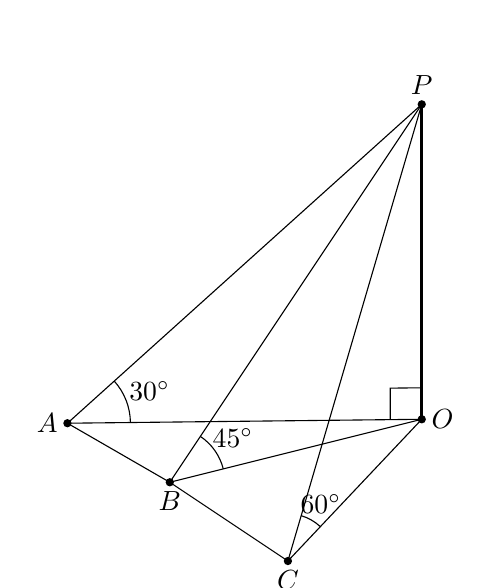
\begin{tikzpicture}[scale=1]
            \coordinate (P) at (5.2,6.8);
            \coordinate (O) at (5.2,2.8);
            \coordinate (A) at (0.7,2.75);
            \coordinate (B) at (2.0,2.0);
            \coordinate (C) at (3.5,1.0);

            \draw (A)--(B)--(C);
            \draw (A)--(O);
            \draw (B)--(O);
            \draw (C)--(O);

            \draw (A)--(P);
            \draw (B)--(P);
            \draw (C)--(P);

            \draw[line width=1pt] (O)--(P);

            \pic[draw,angle radius=4mm]{right angle=A--O--P};

            \pic[draw,"$30^\circ$",angle radius=8mm,angle eccentricity=1.4]{angle=O--A--P};
            \pic[draw,"$45^\circ$",angle radius=7mm,angle eccentricity=1.4]{angle=O--B--P};
            \pic[draw,"$60^\circ$",angle radius=6mm,angle eccentricity=1.4]{angle=O--C--P};

            \fill (A) circle (1.5pt) node[left]{$A$};
            \fill (B) circle (1.5pt) node[below]{$B$};
            \fill (C) circle (1.5pt) node[below]{$C$};
            \fill (O) circle (1.5pt) node[right]{$O$};
            \fill (P) circle (1.5pt) node[above]{$P$};
        \end{tikzpicture}
    \end{center}
    \qscore{4}
\end{question}

\begin{solution}
    求大厦 $OP$ 的高度，已知 $A,B,C$ 共线，$AB=BC=100\text{ m}$，从 $A,B,C$ 测得 $P$ 的仰角分别为 $30^\circ,45^\circ,60^\circ$。\\
    设 $OP=h$，由仰角定义得 $OA,OB,OC$ 关于 $h$ 的表达式；再设 $M$ 为 $O$ 在直线 $ABC$ 上的垂足，$AM=m$，$OM=d$，利用勾股定理建立方程组求 $h$。
    \begin{align*}
        OA=\dfrac{h}{\tan30^\circ}=h\sqrt3, \quad OB=\dfrac{h}{\tan45^\circ}=h, \quad OC=\dfrac{h}{\tan60^\circ}=\dfrac{h}{\sqrt3}
    \end{align*}
    \hfill (1分) \\
    \begin{align*}
        m^2+d^2 &= 3h^2 \\
        (m-100)^2+d^2 &= h^2 \\
        (m-200)^2+d^2 &= \dfrac{h^2}{3}
    \end{align*}
    \hfill (1分) \\
    两式相减消去 $d^2$：
    \begin{align*}
        m^2-(m-100)^2 &= 2h^2 \ \implies\ 100m-5000=h^2 \\
        (m-100)^2-(m-200)^2 &= \dfrac{2h^2}{3} \ \implies\ 300m-45000=h^2
    \end{align*}
    \hfill (1分) \\
    联立解得：
    \begin{align*}
        100m-5000 &= 300m-45000 \\
        m &= 200 \\
        h^2 &= 100(200)-5000 = 15000 \\
        h &= \sqrt{15000} = 50\sqrt6
    \end{align*}
    \hfill (1分)
\end{solution}
%endregion

%region 范围：微积分-指数函数与对数微分法 | 考点：函数定义域、对数微分法 | 难度：中等
\begin{question}[points = 4]
    若函数 $f(x) = x^x$。

    \begin{questionparts}
        \item 求 $f$ 的定义域。 \qscore{1}

        \item 利用对数微分法，求 $f(x)$ 对 $x$ 的导数 $f'(x)$。 \qscore{3}
    \end{questionparts}
\end{question}

\begin{solution}
    \begin{enumerate}[label=(\alph*)]
        \item 求 $f(x) = x^x$ 的定义域。 \\
        由于 $x^x = e^{x\ln x}$，需要 $\ln x$ 有定义。
        \[
            \text{定义域为 } x > 0, \ \text{即 } (0, +\infty)
        \]
        \hfill (1分)

        \item 利用对数微分法求 $f'(x)$。 \\
        对等式 $f(x) = x^x$ 两边取自然对数，再对 $x$ 求导。
        \begin{align*}
            \ln f(x) &= x \ln x
        \end{align*}
        \hfill (1分)
        \begin{align*}
            \frac{d}{dx}\big[\ln f(x)\big] &= \frac{d}{dx}\big[x \ln x\big] \\
            \frac{f'(x)}{f(x)} &= \ln x + x \cdot \frac{1}{x} \\
            \frac{f'(x)}{f(x)} &= \ln x + 1
        \end{align*}
        \hfill (1分)
        \begin{align*}
            f'(x) &= f(x)\big(\ln x + 1\big) \\
            f'(x) &= x^x\big(\ln x + 1\big)
        \end{align*}
        \hfill (1分)
    \end{enumerate}
\end{solution}
%endregion

%region 范围：微积分应用（直线运动） | 考点：分离变量积分求位移、衰减速度模型求瞬时速度 | 难度：中等
\begin{question}[points = 4]
    绍乐一记重杀打出了初速度为 $v_0 = 396\text{ km/h}$的羽球，此后羽球因空气阻力做减速运动，其速度方程为
    \[
        v(t) = \frac{v_0}{1 + kv_0t}, \quad k = 0.03
    \]
    其中 $t$ 的单位为秒（s），速度单位为 $\text{m/s}$。若羽球飞行 $0.1\text{ s}$ 后落地，求：

    \begin{questionparts}
        \item 羽球落地时的速度。 \qscore{1}

        \item 羽球在这 $0.1\text{ s}$ 内飞行的距离。 \qscore{3}
    \end{questionparts}
\end{question}

\begin{solution}
    \begin{enumerate}[label=(\alph*)]
        \item 求羽球飞行 $0.1\text{ s}$ 内的距离。 \\
        位移为速度对时间的积分，先将 $v_0$ 化为 $\text{m/s}$ 制。
        \[
            v_0 = 396\text{ km/h} = \frac{396 \times 1000}{3600}\text{ m/s} = 110\text{ m/s}
        \]
        \hfill (1分)
        \begin{align*}
            s &= \int_0^{0.1} \frac{v_0}{1+kv_0t}\,dt \\
            &= \frac{1}{k}\ln(1+kv_0t)\Big|_0^{0.1} \\
            &= \frac{1}{0.03}\ln(1+0.03\times110\times0.1) \\
            &= \frac{100}{3}\ln(1.33) \\
            &\approx 9.51\text{ m}
        \end{align*}
        \hfill (1分)

        \item 求羽球落地时（$t=0.1\text{ s}$）的速度。 \\
        代入 $t=0.1$ 于速度方程即可。
        \begin{align*}
            v(0.1) &= \frac{v_0}{1+kv_0\times0.1} \\
            &= \frac{110}{1+0.03\times110\times0.1} \\
            &= \frac{110}{1.33} \\
            &\approx 82.71\text{ m/s}
        \end{align*}
        \hfill (1分)
    \end{enumerate}
\end{solution}
%endregion

%region 范围：代数方程与复数根 | 考点：实系数多项式的共轭复根定理、多项式除法、多项式因式分解 | 难度：中等
\begin{question}[points = 6]
    已知复数 $1+i$ 是方程$x^5 - 6x^4 + 11x^3 - 4x^2 - 10x + 12 = 0$的一个根，求此方程的其余四个根。 \qscore{6}
\end{question}

\begin{solution}
    已知 $1+i$ 是该实系数五次方程的一个根，求其余四个根。 \\
    由实系数多项式的共轭根定理与多项式除法逐步降次求解。

    由于方程系数均为实数，复根必成共轭对出现，故 $1-i$ 也是该方程的根。
    \hfill (1分)

    以这一对共轭复根构造二次因式：
    \begin{align*}
        \big(x-(1+i)\big)\big(x-(1-i)\big) &= (x-1)^2 - i^2 \\
        &= x^2 - 2x + 2
    \end{align*}
    \hfill (1分)

    将原五次多项式除以该二次因式，求商式：
    \begin{align*}
        x^5 - 6x^4 + 11x^3 - 4x^2 - 10x + 12 &= (x^2-2x+2)\big(x^3-4x^2+x+6\big)
    \end{align*}
    \hfill (2分)

    对三次商式 $x^3-4x^2+x+6$ 用有理根定理测试，验证 $x=2,-1,3$ 均满足，从而因式分解：
    \begin{align*}
        x^3-4x^2+x+6 &= (x-2)(x+1)(x-3)
    \end{align*}
    \[
        \text{故该方程的其余四个根为 } 1-i,\ 2,\ -1,\ 3
    \]
    \hfill (2分)
\end{solution}
%endregion

% %region 范围：高级数学 31.数学方法 | 考点：数学归纳法（求和公式证明） | 难度：中等
% \begin{question}[points = 6]
%     用数学归纳法证明：
%     \newline
%     对于所有正整数 $n$，
%         $\displaystyle 1\times 2 + 2\times 3 + 3\times 4 + \cdots + n(n+1) = \frac{n(n+1)(n+2)}{3}.$
%     \qscore{6}
% \end{question}

% \begin{solution}
%     证明对所有正整数 $n$，$1\times 2 + 2\times 3 + \cdots + n(n+1) = \dfrac{n(n+1)(n+2)}{3}$。 \\
%     用数学归纳法，先验证 $n=1$ 成立，再证明 $n=k$ 成立可推出 $n=k+1$ 成立。 \\
%     设 $P(n)$ 表示命题：$1\times 2 + 2\times 3 + \cdots + n(n+1) = \dfrac{n(n+1)(n+2)}{3}$。

%     当 $n=1$ 时，
%     \[
%         \text{左边} = 1\times 2 = 2, \qquad \text{右边} = \frac{1\times 2\times 3}{3} = 2.
%     \]
%     左边 $=$ 右边，故 $P(1)$ 成立。
%     \hfill (1分)

%     假设当 $n=k$（$k$ 为正整数）时 $P(k)$ 成立，即
%     \[
%         1\times 2 + 2\times 3 + \cdots + k(k+1) = \frac{k(k+1)(k+2)}{3}.
%     \]
%     \hfill (1分)

%     当 $n=k+1$ 时，
%     \begin{align*}
%         1\times 2 + 2\times 3 + \cdots + k(k+1) + (k+1)(k+2)
%         &= \frac{k(k+1)(k+2)}{3} + (k+1)(k+2)
%     \end{align*}
%     \hfill (1分)
%     \begin{align*}
%         &= \frac{k(k+1)(k+2) + 3(k+1)(k+2)}{3} \\
%         &= \frac{(k+1)(k+2)(k+3)}{3}
%     \end{align*}
%     \hfill (2分)

%     即 $P(k+1)$ 成立。根据数学归纳法原理，$P(n)$ 对所有正整数 $n$ 成立。
%     \hfill (1分)
% \end{solution}
% %endregion
%region 范围：高级数学 31.数学方法 | 考点：数学归纳法（整除性证明） | 难度：困难
\begin{question}[points = 6]
    用数学归纳法证明：对于所有正整数 $n$，$\displaystyle 11^{n+2} + 12^{2n+1}$能被 $133$ 整除。
    \qscore{6}
\end{question}

\begin{solution}
    证明对所有正整数 $n$，$11^{n+2} + 12^{2n+1}$ 能被 $133$ 整除。 \\
    用数学归纳法，关键在于把 $n=k+1$ 时的表达式拆成含归纳假设的项与另一个明显能被 $133$ 整除的项。 \\
    设 $P(n)$ 表示命题：$11^{n+2} + 12^{2n+1} = 133m$（$m$ 为某正整数）。

    当 $n=1$ 时，
    \[
        11^{3} + 12^{3} = 1331 + 1728 = 3059 = 133 \times 23.
    \]
    故 $P(1)$ 成立。
    \hfill (1分)

    假设当 $n=k$（$k$ 为正整数）时 $P(k)$ 成立，即存在正整数 $m$ 使得
    \[
        11^{k+2} + 12^{2k+1} = 133m.
    \]
    \hfill (1分)

    当 $n=k+1$ 时，
    \begin{align*}
        11^{(k+1)+2} + 12^{2(k+1)+1}
        &= 11^{k+3} + 12^{2k+3} \\
        &= 11\cdot 11^{k+2} + 144\cdot 12^{2k+1}
    \end{align*}
    \hfill (1分)
    \begin{align*}
        &= 11\cdot 11^{k+2} + (11+133)\cdot 12^{2k+1} \\
        &= 11\left(11^{k+2} + 12^{2k+1}\right) + 133\cdot 12^{2k+1}
    \end{align*}
    \hfill (2分)

    由归纳假设，$11^{k+2}+12^{2k+1}=133m$，代入得
    \[
        11^{k+3} + 12^{2k+3} = 11(133m) + 133\cdot 12^{2k+1} = 133\left(11m + 12^{2k+1}\right),
    \]
    即 $P(k+1)$ 成立。根据数学归纳法原理，$P(n)$ 对所有正整数 $n$ 成立。
    \hfill (1分)
\end{solution}
%endregion


%region 范围：高中三角函数——多倍角恒等式的证明与应用 | 考点：半角/二倍角公式推导恒等式、并用该恒等式将四倍角方程化为四次方程求解 | 难度：困难
\begin{question}[points = 6]
    \begin{questionparts}
        \item 证明 $\dfrac18\cos4x+\dfrac12\cos2x+\dfrac38=\cos^4x$。 \qscore{3}

        \item 据此，或用其他方法，解方程 $\cos4x+4\cos2x=-1$，其中 $0\leq x\leq2\pi$。 \qscore{3}
    \end{questionparts}
\end{question}

\begin{solution}
    \begin{enumerate}[label=(\alph*)]
        \item 证明 $\dfrac18\cos4x+\dfrac12\cos2x+\dfrac38=\cos^4x$。\\
        将 $\cos^4x$ 写成 $\left(\dfrac{1+\cos2x}{2}\right)^2$ 后展开，再用二倍角公式把 $\cos^22x$ 化为含 $\cos4x$ 的式子。
        \begin{align*}
            \cos^4x &= \left(\dfrac{1+\cos2x}{2}\right)^2 \\
            &= \dfrac{1+2\cos2x+\cos^22x}{4}
        \end{align*}
        \hfill (1分) \\
        \begin{align*}
            \cos^22x &= \dfrac{1+\cos4x}{2}
        \end{align*}
        \hfill (1分) \\
        \begin{align*}
            \cos^4x &= \dfrac{1+2\cos2x+\dfrac{1+\cos4x}{2}}{4} \\
            &= \dfrac38+\dfrac12\cos2x+\dfrac18\cos4x
        \end{align*}
        \hfill (1分)

        \item 解方程 $\cos4x+4\cos2x=-1$，$0\leq x\leq2\pi$。\\
        由 (a) 的恒等式得 $\cos4x=8\cos^4x-4\cos2x-3$，代入原方程消去 $\cos4x$ 化为关于 $\cos^4x$ 的方程求解。
        \begin{align*}
            8\cos^4x-4\cos2x-3+4\cos2x &= -1 \\
            8\cos^4x &= 2 \\
            \cos^4x &= \dfrac14
        \end{align*}
        \hfill (1分) \\
        \begin{align*}
            \cos^2x &= \dfrac12 \quad(\text{舍去负值}) \\
            \cos x &= \pm\dfrac{\sqrt2}{2}
        \end{align*}
        \hfill (1分) \\
        在 $0\leq x\leq2\pi$ 范围内：
        \[
            x = \dfrac{\pi}{4},\ \dfrac{3\pi}{4},\ \dfrac{5\pi}{4},\ \dfrac{7\pi}{4}
        \]
        \hfill (1分)
    \end{enumerate}
\end{solution}
%endregion

%region 范围：高级数学 35.空间向量 | 考点：向量的内积（求夹角）与外积（求面积） | 难度：中等
\begin{question}[points = 6]
    已知平行四边形 $PQRS$ 的其中三个顶点为 $P(2,-1,3)$、$Q(4,0,5)$ 及 $R(5,2,3)$。

    \begin{questionparts}
        \item 求 $\overrightarrow{PQ}$ 与 $\overrightarrow{PR}$ 之间的夹角。 \qscore{3}

        \item 求平行四边形 $PQRS$ 的面积。 \qscore{3}
    \end{questionparts}
\end{question}

\begin{solution}
    \begin{enumerate}[label=(\alph*)]
        \item 求 $\overrightarrow{PQ}$ 与 $\overrightarrow{PR}$ 之间的夹角。 \\
        先求出两向量，再利用内积公式 $\cos\theta = \dfrac{\overrightarrow{PQ}\cdot\overrightarrow{PR}}{|\overrightarrow{PQ}||\overrightarrow{PR}|}$ 求解。 \\
        \[
            \overrightarrow{PQ} = (2,1,2), \qquad \overrightarrow{PR} = (3,3,0)
        \]
        \hfill (1分)
        \[
            \overrightarrow{PQ}\cdot\overrightarrow{PR} = (2)(3)+(1)(3)+(2)(0) = 9, \qquad |\overrightarrow{PQ}| = 3, \qquad |\overrightarrow{PR}| = 3\sqrt{2}
        \]
        \hfill (1分)
        \[
            \cos\theta = \frac{9}{3\times 3\sqrt{2}} = \frac{1}{\sqrt{2}} \quad\Rightarrow\quad \theta = 45^\circ
        \]
        \hfill (1分)

        \item 求平行四边形 $PQRS$ 的面积。 \\
        面积等于以 $\overrightarrow{PQ}$、$\overrightarrow{QR}$ 为邻边所张成的 $|\overrightarrow{PQ}\times\overrightarrow{QR}|$。 \\
        \[
            \overrightarrow{QR} = (1,2,-2)
        \]
        \hfill (1分)
        \begin{align*}
            \overrightarrow{PQ}\times\overrightarrow{QR}
            &= \begin{vmatrix} \vec{i} & \vec{j} & \vec{k} \\ 2 & 1 & 2 \\ 1 & 2 & -2 \end{vmatrix} \\
            &= \vec{i}\big((1)(-2)-(2)(2)\big) - \vec{j}\big((2)(-2)-(2)(1)\big) + \vec{k}\big((2)(2)-(1)(1)\big) \\
            &= (-6,\,6,\,3)
        \end{align*}
        \hfill (1分)
        \[
            \text{面积} = |\overrightarrow{PQ}\times\overrightarrow{QR}| = \sqrt{(-6)^2+6^2+3^2} = \sqrt{81} = 9
        \]
        \hfill (1分)
    \end{enumerate}
\end{solution}
%endregion
% %region 范围：平面/空间向量 | 考点：向量数量积的展开与最值分析、由数量积反求夹角 | 难度：中等
% \begin{question}[points = 6]
%     若 $\underline{a}$ 与 $\underline{b}$ 均为单位向量。

%     \begin{questionparts}
%         \item 求 $(\underline{a}+\underline{b})\cdot(\underline{a}-2\underline{b})$ 的最大可能值及最小可能值。 \qscore{3}

%         \item 若 $(\underline{a}+\underline{b})\cdot(\underline{a}-2\underline{b}) = -\dfrac{3}{2}$，求 $\underline{a}$ 与 $\underline{b}$ 的夹角。 \qscore{3}
%     \end{questionparts}
% \end{question}

% \begin{solution}
%     设 $\underline{a}$ 与 $\underline{b}$ 的夹角为 $\theta$，则 $\underline{a}\cdot\underline{b}=|\underline{a}||\underline{b}|\cos\theta=\cos\theta$（因为 $|\underline{a}|=|\underline{b}|=1$）。

%     先展开 $(\underline{a}+\underline{b})\cdot(\underline{a}-2\underline{b})$：
%     \begin{align*}
%         (\underline{a}+\underline{b})\cdot(\underline{a}-2\underline{b})
%         &= \underline{a}\cdot\underline{a} - 2\underline{a}\cdot\underline{b} + \underline{b}\cdot\underline{a} - 2\underline{b}\cdot\underline{b} \\
%         &= |\underline{a}|^2 - \underline{a}\cdot\underline{b} - 2|\underline{b}|^2 \\
%         &= 1 - \cos\theta - 2 \\
%         &= -1 - \cos\theta
%     \end{align*}
%     \hfill (共用展开，不单独计分)

%     \begin{enumerate}[label=(\alph*)]
%         \item 求最大值和最小值。 \\
%         因为 $\theta\in[0,\pi]$，所以 $\cos\theta\in[-1,1]$。 \\
%         \hfill (1分)

%         \begin{align*}
%             \text{当 } \cos\theta = -1 \text{（即 }\theta=\pi\text{）时，}\quad
%             -1-\cos\theta = -1-(-1) = 0 \quad \text{（最大值）}
%         \end{align*}
%         \hfill (1分)

%         \begin{align*}
%             \text{当 } \cos\theta = 1 \text{（即 }\theta=0\text{）时，}\quad
%             -1-\cos\theta = -1-1 = -2 \quad \text{（最小值）}
%         \end{align*}
%         \hfill (1分)

%         \item 求夹角。 \\
%         由 (a) 的展开式，令
%         \[
%             -1-\cos\theta = -\frac{3}{2}
%         \]
%         \hfill (1分)

%         解得
%         \[
%             \cos\theta = -\frac{3}{2}+1... 
%         \]
%         (整理：$-\cos\theta = -\dfrac32+1=-\dfrac12$，即)
%         \[
%             \cos\theta = \frac{1}{2}
%         \]
%         \hfill (1分)

%         因为 $\theta\in[0,\pi]$，所以
%         \[
%             \theta = \frac{\pi}{3}\ (\text{即}\ 60^\circ)
%         \]
%         \hfill (1分)
%     \end{enumerate}
% \end{solution}
% %endregion


% %region 范围：空间向量 | 考点：向量的数量积（内积）求夹角、向量的向量积（外积）求平行四边形面积 | 难度：中等
% \begin{question}[points = 6]
%     已知空间向量 $\vec{a} = (1,1,0)$，$\vec{b} = (1,0,1)$。

%     \begin{questionparts}
%         \item 求 $\vec{a}\cdot\vec{b}$（内积），并求 $\vec{a}$ 与 $\vec{b}$ 之间夹角 $\theta$ 的余弦值。 \qscore{3}

%         \item 求 $\vec{a}\times\vec{b}$（外积），并求以 $\vec{a}$、$\vec{b}$ 为邻边的平行四边形的面积。 \qscore{3}
%     \end{questionparts}
% \end{question}

% \begin{solution}
%     \begin{enumerate}[label=(\alph*)]
%         \item 求内积并求夹角余弦值。 \\
%         由数量积定义
%         \[
%             \vec{a}\cdot\vec{b} = 1\times1 + 1\times0 + 0\times1 = 1
%         \]
%         \hfill (1分)

%         又
%         \[
%             |\vec{a}| = \sqrt{1^2+1^2+0^2} = \sqrt{2}, \qquad
%             |\vec{b}| = \sqrt{1^2+0^2+1^2} = \sqrt{2}
%         \]
%         \hfill (1分)

%         所以
%         \[
%             \cos\theta = \frac{\vec{a}\cdot\vec{b}}{|\vec{a}||\vec{b}|} = \frac{1}{\sqrt2\times\sqrt2} = \frac{1}{2}
%         \]
%         \hfill (1分)

%         \item 求外积并求平行四边形面积。 \\
%         由向量积的行列式公式
%         \[
%             \vec{a}\times\vec{b} =
%             \begin{vmatrix}
%                 \vec{i} & \vec{j} & \vec{k} \\
%                 1 & 1 & 0 \\
%                 1 & 0 & 1
%             \end{vmatrix}
%         \]
%         \hfill (1分)

%         展开得
%         \begin{align*}
%             \vec{a}\times\vec{b}
%             &= \vec{i}(1\times1-0\times0) - \vec{j}(1\times1-0\times1) + \vec{k}(1\times0-1\times1) \\
%             &= (1,\,-1,\,-1)
%         \end{align*}
%         \hfill (1分)

%         平行四边形的面积等于外积的模长，即
%         \[
%             S = |\vec{a}\times\vec{b}| = \sqrt{1^2+(-1)^2+(-1)^2} = \sqrt{3}
%         \]
%         \hfill (1分)
%     \end{enumerate}
% \end{solution}
% %endregion

%region 范围：解析几何——抛物线的参数表示、轨迹方程与焦点 | 考点：抛物线参数方程、中点轨迹消参、标准式配方求焦点 | 难度：中等
\begin{question}[points = 6]
    设 $P$ 为抛物线 $y^2=8x$ 上的一动点，$Q$ 为定点，坐标为 $(p,q)$。

    \begin{questionparts}
        \item 证明线段 $PQ$ 的中点 $M$ 的轨迹方程为$\displaystyle \left(x-\frac{p}{2}\right)=\left(y-\frac{q}{2}\right)^2$。\qscore{3}

        \item 求 (a) 小题中所得曲线的焦点坐标。 \qscore{3}
    \end{questionparts}
\end{question}

\begin{solution}
    \begin{enumerate}[label=(\alph*)]
        \item 证明中点 $M$ 的轨迹方程。 \\
        抛物线 $y^2=8x$ 可用参数表示，设 $P$ 对应参数 $t$。

        设 $P=(2t^2,4t)$，验证 $(4t)^2=16t^2=8(2t^2)$，符合方程。
        \hfill (1分)

        设 $M(x,y)$ 为 $PQ$ 的中点，由中点公式：
        \begin{align*}
            x &=\frac{2t^2+p}{2}=t^2+\frac{p}{2} \\
            y &=\frac{4t+q}{2}=2t+\frac{q}{2}
        \end{align*}
        \hfill (1分)

        由第二式解出 $t=\dfrac{1}{2}\left(y-\dfrac{q}{2}\right)$，代入第一式消去 $t$：
        \begin{align*}
            x-\frac{p}{2} &=t^2 \\
            &=\left[\frac{1}{2}\left(y-\frac{q}{2}\right)\right]^2 \\
            &=\frac{1}{4}\left(y-\frac{q}{2}\right)^2
        \end{align*}
        即
        \[
            4\left(x-\frac{p}{2}\right)=\left(y-\frac{q}{2}\right)^2.
        \]
        \hfill (1分)

        \item 求曲线 $4\left(x-\dfrac{p}{2}\right)=\left(y-\dfrac{q}{2}\right)^2$ 的焦点坐标。 \\
        将曲线化为标准式，通过平移坐标轴消去常数项，与 $Y^2=4aX$ 比较求出 $a$，再换回原坐标。

        设 $X=x-\dfrac{p}{2}$，$Y=y-\dfrac{q}{2}$，则曲线化为
        \[
            Y^2=4X.
        \]
        \hfill (1分)

        与标准式 $Y^2=4aX$ 比较，得 $4a=4$，即 $a=1$，故在 $(X,Y)$ 坐标系中焦点为
        \[
            (X,Y)=(1,0).
        \]
        \hfill (1分)

        换回原坐标 $x=X+\dfrac{p}{2}$，$y=Y+\dfrac{q}{2}$，得焦点坐标为
        \[
            \left(\frac{p}{2}+1,\ \frac{q}{2}\right).
        \]
        \hfill (1分)
    \end{enumerate}
\end{solution}
%endregion


%region 范围：微积分-函数性态分析（渐近线、单调性、极值、凹凸性与拐点） | 考点：极限求渐近线、一阶导数判断单调性与极值、二阶导数判断凹凸性与拐点 | 难度：中等
\begin{question}[points = 10]
    已知函数 $\displaystyle f(x) = \frac{4x}{x^2+1}$。

    \begin{questionparts}
        \item 求曲线 $y = f(x)$ 的水平渐近线。 \qscore{2}

        \item 判断 $f(x)$ 在哪些区间内递增或递减，并据此求出 $f(x)$ 的极值，说明它是极大值或极小值。 \qscore{4}

        \item 求 $f(x)$ 的凸向区间与拐点。 \qscore{4}
    \end{questionparts}
\end{question}

\begin{solution}
    \begin{enumerate}[label=(\alph*)]
        \item 求 $\displaystyle f(x)=\frac{4x}{x^2+1}$ 的水平渐近线。 \\
        考察 $x \to \pm\infty$ 时 $f(x)$ 的极限。
        \begin{align*}
            \lim_{x\to\infty} \frac{4x}{x^2+1} &= \lim_{x\to\infty} \frac{4/x}{1+1/x^2} = 0 \\
            \lim_{x\to-\infty} \frac{4x}{x^2+1} &= 0
        \end{align*}
        \hfill (1分)
        \[
            \text{故曲线 } y=f(x) \text{ 的水平渐近线为 } y=0
        \]
        \hfill (1分)

        \item 判断 $f(x)$ 的单调区间并求极值。 \\
        先求 $f'(x)$，再分析其符号。
        \begin{align*}
            f'(x) &= \frac{4(x^2+1) - 4x(2x)}{(x^2+1)^2} \\
            &= \frac{4-4x^2}{(x^2+1)^2} = \frac{4(1-x)(1+x)}{(x^2+1)^2}
        \end{align*}
        \hfill (1分)
        由于分母恒正，令 $f'(x)=0$ 得驻点 $x=-1, x=1$，分析各区间符号：
        \[
            f'(x) < 0 \text{ 于 } (-\infty,-1), \quad f'(x) > 0 \text{ 于 } (-1,1), \quad f'(x) < 0 \text{ 于 } (1,+\infty)
        \]
        故 $f(x)$ 在 $(-\infty,-1)$ 与 $(1,+\infty)$ 上递减，在 $(-1,1)$ 上递增。
        \hfill (1分)
        \[
            f(-1) = \frac{4(-1)}{(-1)^2+1} = -2
        \]
        由递减转为递增，故 $f$ 在 $x=-1$ 处取得极小值 $f(-1) = -2$。
        \hfill (1分)
        \[
            f(1) = \frac{4(1)}{1^2+1} = 2
        \]
        由递增转为递减，故 $f$ 在 $x=1$ 处取得极大值 $f(1) = 2$。
        \hfill (1分)

        \item 求 $f(x)$ 的凹凸区间与拐点。 \\
        对 $f'(x)$ 再求导得 $f''(x)$。
        \begin{align*}
            f''(x) &= \frac{-8x(x^2+1)^2 - (4-4x^2)\cdot 2(x^2+1)(2x)}{(x^2+1)^4} \\
            &= \frac{-8x(x^2+1) - 4x(4-4x^2)}{(x^2+1)^3} \\
            &= \frac{-8x^3-8x-16x+16x^3}{(x^2+1)^3} \\
            &= \frac{8x^3-24x}{(x^2+1)^3} = \frac{8x(x^2-3)}{(x^2+1)^3}
        \end{align*}
        \hfill (1分)
        由于分母恒正，令 $f''(x)=0$ 得 $x=-\sqrt3,\ 0,\ \sqrt3$，分析各区间符号：
        \[
            f''(x)<0 \text{ 于 } (-\infty,-\sqrt3), \quad f''(x)>0 \text{ 于 } (-\sqrt3,0), \quad f''(x)<0 \text{ 于 } (0,\sqrt3), \quad f''(x)>0 \text{ 于 } (\sqrt3,+\infty)
        \]
        故 $f(x)$ 在 $(-\infty,-\sqrt3)$ 与 $(0,\sqrt3)$ 上为凹向下（凸），在 $(-\sqrt3,0)$ 与 $(\sqrt3,+\infty)$ 上为凹向上（凹）。
        \hfill (1分)
        由于 $f''(x)$ 在 $x=-\sqrt3, 0, \sqrt3$ 处均变号，故这三点均为拐点，计算对应函数值：
        \begin{align*}
            f(-\sqrt3) &= \frac{4(-\sqrt3)}{3+1} = -\sqrt3 \\
            f(0) &= 0 \\
            f(\sqrt3) &= \frac{4\sqrt3}{3+1} = \sqrt3
        \end{align*}
        \hfill (2分)
        \[
            \text{故拐点为 } (-\sqrt3, -\sqrt3),\ (0,0),\ (\sqrt3, \sqrt3)
        \]
    \end{enumerate}
\end{solution}
%endregion

\newpage

%region 范围：不定积分分部积分递推公式与旋转体体积（选自2013年第10(b)题、2014年第11题） | 考点：分部积分递推公式、垫圈法（旋转体体积） | 难度：困难
\begin{question}[points = 10]
    

    \begin{questionparts}
        \item 若 $m$ 与 $n$ 均为正整数，证明 
        $\displaystyle \int x^m(\ln x)^n\,dx=\frac{x^{m+1}}{m+1}(\ln x)^n-\frac{n}{m+1}\int x^m(\ln x)^{n-1}\,dx$，
        据此，求 $\displaystyle\int x\ln x\,dx$ 及 $\displaystyle\int x^2(\ln x)^2\,dx$。 \qscore{5}
\vspace{2pt}
        \item
        \begin{minipage}[t]{0.54\linewidth}
            图中阴影部分是由曲线 $y=x\ln x$，直线 $x=e$ 及 $x$ 轴所围成的区域。若此阴影区域绕直线 $y=-1$ 旋转 $360^\circ$ 后所形成的旋转体体积为 $V$，利用 (a) 的结果，证明下式。$\displaystyle V=\left(\frac{5}{27}e^3+\frac{1}{2}e^2+\frac{23}{54}\right)\pi.$
        \end{minipage}%
        \hfill
        \begin{minipage}[t]{0.44\linewidth}
            \centering
            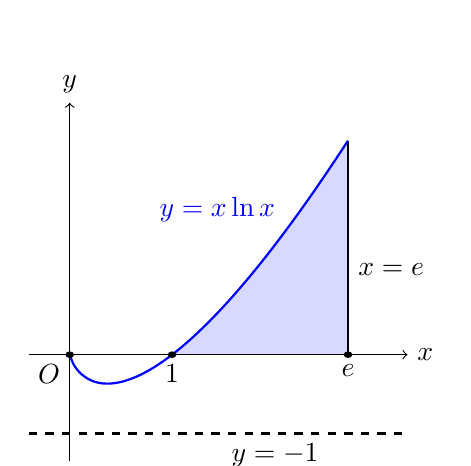
\begin{tikzpicture}[xscale=1.3,yscale=1.0,baseline={([yshift=-\ht\strutbox]current bounding box.north)}]
                % 先画阴影，再画边界，避免遮盖曲线。
                \fill[blue!15] (1,0) -- plot[domain=1:2.71828, smooth, samples=80] ({\x}, {\x*ln(\x)}) -- (2.71828,0) -- cycle;

                \draw[->] (-0.4,0) -- (3.3,0) node[right] {$x$};
                \draw[->] (0,-1.35) -- (0,3.2) node[above] {$y$};

                % 旋转轴及区域的右边界。
                \draw[dashed,thick] (-0.4,-1) -- (3.3,-1)
                    node[pos=0.65,below] {$y=-1$};
                \draw[thick] (2.71828,0) -- (2.71828,2.71828)
                    node[pos=0.4,right] {$x=e$};
                \draw[domain=0.001:2.71828, smooth, samples=80, thick, blue]
                    plot ({\x}, {\x*ln(\x)});
                \node[blue,above left] at (2.1,{2.1*ln(2.1)}) {$y=x\ln x$};

                \coordinate (O) at (0,0);
                \coordinate (A) at (1,0);
                \coordinate (E) at (2.71828,0);
                \fill (O) circle (1.2pt) node[below left] {$O$};
                \fill (A) circle (1.2pt) node[below] {$1$};
                \fill (E) circle (1.2pt) node[below] {$e$};
            \end{tikzpicture}
        \end{minipage}

        \qscore{5}
    \end{questionparts}
\end{question}

\begin{solution}
    \begin{enumerate}[label=(\alph*)]
        \item 证明分部积分递推公式并求出两个不定积分。 \\
        取 $u=(\ln x)^n$，$dv=x^m\,dx$，则 $du=\dfrac{n(\ln x)^{n-1}}{x}\,dx$，$v=\dfrac{x^{m+1}}{m+1}$，代入分部积分公式：
        \[
            \int x^m(\ln x)^n\,dx=\frac{x^{m+1}}{m+1}(\ln x)^n-\frac{n}{m+1}\int x^m(\ln x)^{n-1}\,dx.
        \]
        \hfill (2分)

        取 $m=1,\ n=1$：
        \begin{align*}
            \int x\ln x\,dx &=\frac{x^2}{2}\ln x-\frac{1}{2}\int x\,dx \\
            &=\frac{x^2}{2}\ln x-\frac{x^2}{4}+C
        \end{align*}
        \hfill (1分)

        取 $m=2,\ n=2$，再取 $m=2,\ n=1$ 求出 $\displaystyle\int x^2\ln x\,dx=\frac{x^3}{3}\ln x-\frac{x^3}{9}+C$，代回：
        \begin{align*}
            \int x^2(\ln x)^2\,dx &=\frac{x^3}{3}(\ln x)^2-\frac{2}{3}\int x^2\ln x\,dx \\
            &=\frac{x^3}{3}(\ln x)^2-\frac{2}{3}\left(\frac{x^3}{3}\ln x-\frac{x^3}{9}\right)+C \\
            &=\frac{x^3}{3}(\ln x)^2-\frac{2x^3}{9}\ln x+\frac{2x^3}{27}+C
        \end{align*}
        \hfill (2分)

        \item 求阴影区域绕 $y=-1$ 旋转所得旋转体体积 $V$。 \\
        阴影区域为 $1\le x\le e$、上界 $y=x\ln x$、下界 $y=0$ 所围成的部分，用垫圈法计算。

        外半径 $R(x)=x\ln x+1$，内半径 $r(x)=1$：
        \[
            V=\pi\int_1^e\Big[(x\ln x+1)^2-1^2\Big]\,dx=\pi\int_1^e\Big[x^2(\ln x)^2+2x\ln x\Big]\,dx
        \]
        \hfill (1分)

        代入 (a) 所得结果，令
        \[
            F(x)=\frac{x^3}{3}(\ln x)^2-\frac{2x^3}{9}\ln x+\frac{2x^3}{27}+x^2\ln x-\frac{x^2}{2}
        \]
        \hfill (1分)

        当 $x=e$（$\ln e=1$）：
        \begin{align*}
            F(e) &=\frac{e^3}{3}-\frac{2e^3}{9}+\frac{2e^3}{27}+e^2-\frac{e^2}{2} \\
            &=\frac{5e^3}{27}+\frac{e^2}{2}
        \end{align*}
        \hfill (1分)

        当 $x=1$（$\ln 1=0$）：
        \[
            F(1)=\frac{2}{27}-\frac{1}{2}=-\frac{23}{54}
        \]
        \hfill (1分)

        故
        \begin{align*}
            V &=\pi\big[F(e)-F(1)\big] \\
            &=\pi\left[\frac{5e^3}{27}+\frac{e^2}{2}+\frac{23}{54}\right] \\
            &=\left(\frac{5}{27}e^3+\frac{1}{2}e^2+\frac{23}{54}\right)\pi
        \end{align*}
        \hfill (1分)
    \end{enumerate}
\end{solution}
%endregion

\vfill % 与上方内容保持距离

\noindent
\newlength{\sigwidth}
\settowidth{\sigwidth}{（\hspace{4em}师）}

\begin{tabular*}{\textwidth}{@{\extracolsep{\fill}} l l l}
    出题： & 审题： & 审核： \\[4em]
    \rule{\sigwidth}{0.5pt} &
    \rule{\sigwidth}{0.5pt} &
    \rule{\sigwidth}{0.5pt} \\
    （\hspace{0em} \setterteacher ） &
    （\hspace{0em} \reviewteacher ）  &
    （\hspace{0em} \auditteacher ） \\
\end{tabular*}

\clearpage
\thispagestyle{empty} % 取消这一页的页眉页脚（页码）
~
\clearpage
\end{document}
